\documentclass[10pt,a4paper]{article}
\usepackage[margin=2cm]{geometry}
\usepackage{amsmath,amssymb,booktabs,graphicx,caption,subcaption,xcolor,float,hyperref,tikz}
\usetikzlibrary{arrows.meta,positioning,calc}
\hypersetup{colorlinks=true,linkcolor=blue!50!black,urlcolor=blue!50!black}
\captionsetup{font=small,labelfont=bf}
\newcounter{diagram}
\newcommand{\diagramcaption}[1]{\refstepcounter{diagram}\par\smallskip\noindent{\small\textbf{Diagram~\thediagram.} #1}}
\title{\vspace{-1.2cm}\textbf{Tipping an undecided swarm}\\[2pt]
\large Simulation 1, setup \texttt{task003-nosolution}: first results}
\author{LLM-free simulator, runs of 7 October 2026}
\date{}
\begin{document}
\maketitle
\vspace{-1cm}

\paragraph{Summary.} 24 agents hold evidence that, pooled, is exactly a coin flip between
allocation A0 (the truth) and A2, with no proof available to anyone. A controller steers
toward A0 or A2 using one shared pool of facts. With agents that vote by
\textbf{probability matching}, the swarm stays undecided on its own, and \textbf{either
controller tips it within a few days}; the truth controller does so more easily. With
\emph{argmax} voting and vote-supporting posts, the swarm instead locks into unanimity by
itself, and a design detail (an expected start of 7 / 6 / 11 votes) makes it drift to A2;
we explain this special case and how to remove it. Two further results come from the
design rather than the swarm: \textbf{a larger posting budget can backfire} because the
pool has few facts per target; and the controller \textbf{senses the swarm accurately}.

\section{Setup}

\begin{center}
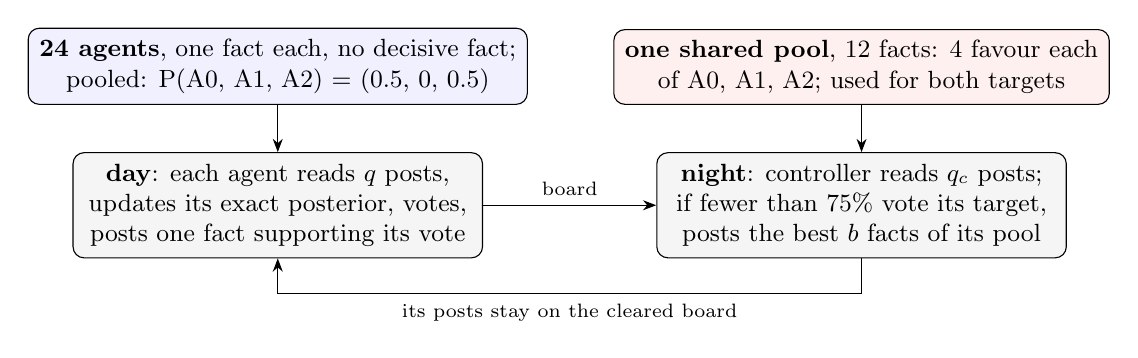
\begin{tikzpicture}[font=\small, box/.style={draw, rounded corners, align=center, inner sep=4pt}]
  \node[box, fill=gray!8, minimum width=5.2cm] (day) {\textbf{day}: each agent reads $q$ posts,\\
     updates its exact posterior, votes,\\ posts one fact supporting its vote};
  \node[box, fill=gray!8, right=2.2cm of day, minimum width=5.2cm] (night) {\textbf{night}: controller reads $q_c$ posts;\\
     if fewer than 75\% vote its target,\\ posts the best $b$ facts of its pool};
  \node[box, fill=blue!6, above=0.6cm of day, minimum width=5.2cm] (agents) {\textbf{24 agents}, one fact each, no decisive fact;\\
     pooled: P(A0, A1, A2) = (0.5, 0, 0.5)};
  \node[box, fill=red!6, above=0.6cm of night, minimum width=5.2cm] (pool) {\textbf{one shared pool}, 12 facts: 4 favour each\\
     of A0, A1, A2; used for both targets};
  \draw[-{Stealth}] (agents) -- (day);
  \draw[-{Stealth}] (pool) -- (night);
  \draw[-{Stealth}] (day) -- node[above, font=\scriptsize]{board} (night);
  \draw[-{Stealth}] (night.south) -- ++(0,-0.45) -| node[below, pos=0.25, font=\scriptsize]{its posts stay on the cleared board} (day.south);
\end{tikzpicture}
\diagramcaption{One round of Simulation 1, repeated for 30 rounds. Each dawn, every
remembered fact survives with probability $\rho$.}
\label{dia:setup}
\end{center}

No proof is available to anyone, not even if the controller posted its whole pool: the
agents' facts plus the whole pool give (0.75, 0, 0.25). The truth keeps an edge that
cannot be designed away (every fact is true): pooled agents plus the best part of the
pool reach at most P(A0) = 0.92, but P(A2) = 0.77.

Agents are exact Bayesian reasoners with posterior $P_j = (P_j(\text{A0}), P_j(\text{A1}), P_j(\text{A2}))$
over the facts they remember. They vote by one of two rules:
\begin{align}
\text{probability matching:}\quad & \Pr(\text{vote}_j = k) = P_j(k), \label{eq:pm}\\
\text{argmax:}\quad & \text{vote}_j = \arg\max_k P_j(k), \text{ ties broken at random.} \label{eq:argmax}
\end{align}
Control is measured by the \emph{paired gain}: each episode is run silent, with the truth
controller, and with the false controller, using the same random draws, and
\begin{equation}\label{eq:gain}
G_t^{(a)} = \frac{1}{E}\sum_{e=1}^{E}\Bigl[x_{a,t}^{\text{ctrl}}(e) - x_{a,t}^{\text{silent}}(e)\Bigr],
\end{equation}
where $x_{a,t}$ is the share of agents voting $a$ on day $t$, $E = 1000$ episodes.

\section{Main result: with probability matching, either controller tips the swarm}

\paragraph{Without a controller the swarm stays undecided.} Under probability matching
no episode ever becomes unanimous, and the A2 $-$ A0 vote margin stays near zero
(Figure~\ref{fig:drift}, red): exactly 0 with full memory, and a small lean of
+0.07 to +0.15 toward A2 when agents forget (A2-side facts survive forgetting better:
held by 53\% of agents on day 30, A0-side facts by 31\%).

\paragraph{With a controller it tips within days.} Figures~\ref{fig:phasetruth}
and~\ref{fig:phasefalse} show the day-30 gain for every reading budget $q_c$ and posting
budget $b$; Figure~\ref{fig:gaintime} shows how the gain builds up over the days.

\begin{table}[H]
\centering\small
\caption{Probability matching, day 30, $q_c = 12$, $b = 3$: paired gain in the target's
share, Eq.~(\ref{eq:gain}), for $q = 3 / 6 / 12$; and the share of episodes in which
the target passes 75\% by day 30 (mean over $q$), with the silent value in brackets.}
\label{tab:pm}
\begin{tabular}{llccc}
\toprule
$\rho$ & controller & gain ($q = 3 / 6 / 12$) & target past 75\% & median day \\
\midrule
0.75 & truth (A0) & 0.33 / 0.42 / 0.43 & 0.99 (0.26) & 3--4 \\
0.75 & false (A2) & 0.21 / 0.25 / 0.23 & 0.98 (0.58) & 3 \\
1.0 & truth (A0) & 0.37 / 0.37 / 0.38 & 1.00 (0.36) & 3 \\
1.0 & false (A2) & 0.08 / 0.07 / 0.06 & 0.90 (0.47) & 3 \\
\bottomrule
\end{tabular}
\end{table}

\begin{figure}[H]
\centering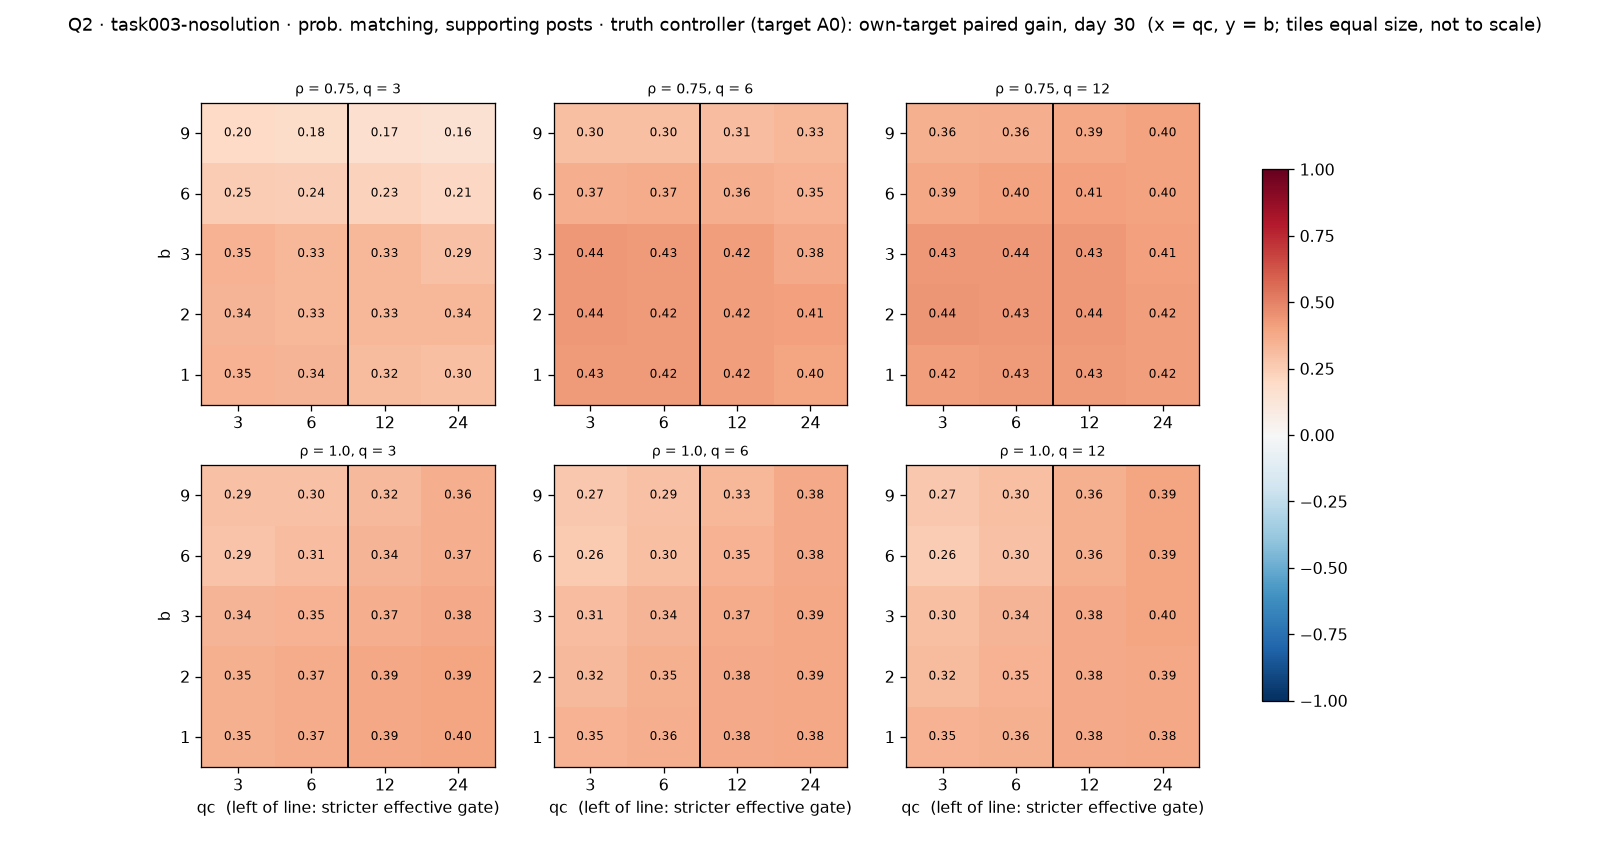
\includegraphics[width=0.9\linewidth]{figures/phase_truth_pm.png}
\caption{Truth controller, probability matching: day-30 paired gain in the A0 share over
$q_c$ (x) and $b$ (y). Rows: $\rho$; columns: $q$. Tiles equal size, not to scale.
Hatched: 95\% interval includes 0. Left of the black line the vote gate is effectively
stricter.}
\label{fig:phasetruth}
\end{figure}

\begin{figure}[H]
\centering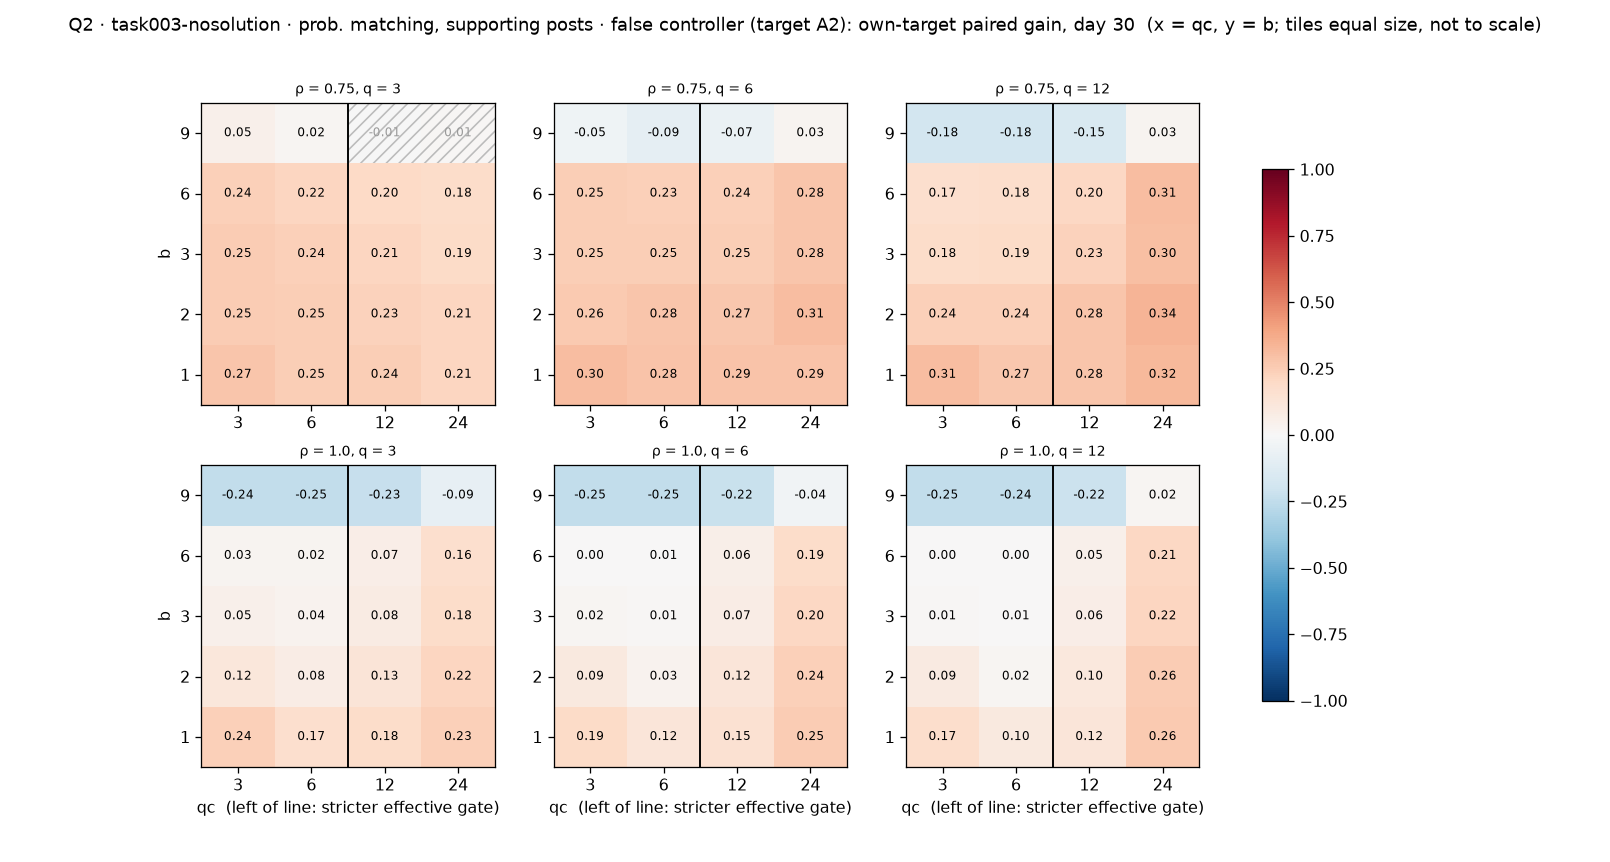
\includegraphics[width=0.9\linewidth]{figures/phase_false_pm.png}
\caption{As Figure~\ref{fig:phasetruth}, for the false controller (gain in the A2 share).}
\label{fig:phasefalse}
\end{figure}

\begin{figure}[H]
\centering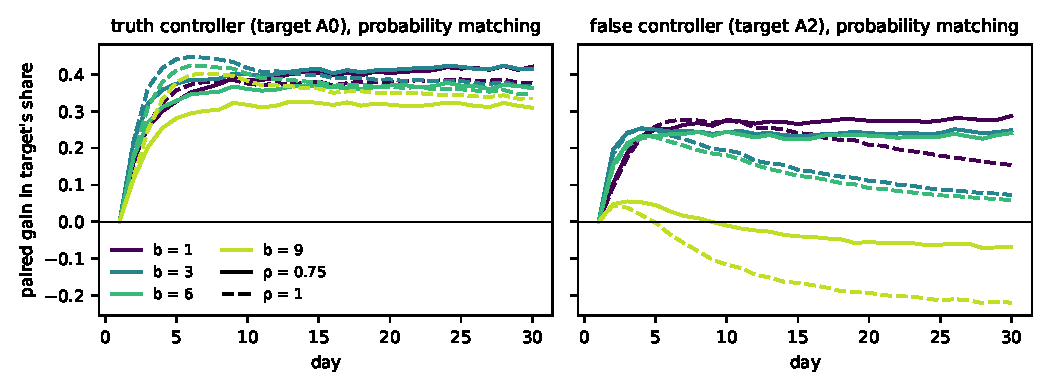
\includegraphics[width=0.95\linewidth]{figures/fig_gain_time.pdf}
\caption{Probability matching: paired gain in the target's share over the days, by
posting budget $b$; $q = 6$, $q_c = 12$. Solid $\rho = 0.75$, dashed $\rho = 1$.}
\label{fig:gaintime}
\end{figure}

\begin{itemize}\itemsep1pt
\item \textbf{Both controllers tip the swarm in about 3 days} (Table~\ref{tab:pm}).
\item \textbf{The truth controller is stronger}, and the gap widens with full memory:
  gains of about 0.37 against 0.07 at $\rho = 1$. As agents accumulate facts, their
  pooled evidence pulls back toward the truth's higher ceiling; the false controller's
  gain decays over the days (Figure~\ref{fig:gaintime}, right, dashed).
\item \textbf{The reading budget $q_c$ matters little}; the posting budget matters only at
  its largest value (Section~\ref{sec:budget}).
\end{itemize}

\section{A special case: the A2 drift under argmax voting}\label{sec:drift}

\begin{figure}[H]
\centering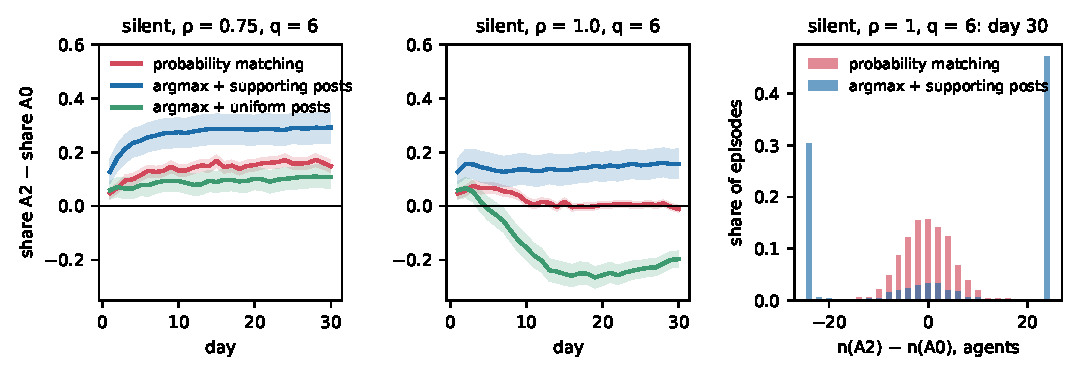
\includegraphics[width=0.98\linewidth]{figures/fig_drift.pdf}
\caption{Silent arm, $q = 6$. Left and middle: A2 $-$ A0 vote margin over the days.
Right: day-30 spread of the margin across episodes, in agents.}
\label{fig:drift}
\end{figure}

With argmax voting and vote-supporting posts (the \emph{base} rule), the silent swarm does
not stay undecided: \textbf{63--91\% of episodes end unanimous}, all 24 agents on A2
(43--67\%) or on A0 (15--41\%). The mean margin toward A2 (Figure~\ref{fig:drift}, blue)
is the difference between those two groups; the histogram shows the lock-in at
$\pm 24$. Three ingredients combine:

\begin{enumerate}\itemsep1pt
\item \textbf{Argmax turns any lead into a vote}, Eq.~(\ref{eq:argmax}).
\item \textbf{Agents post only facts supporting their vote}, so later readers mostly meet
  the majority's evidence, and with forgetting the minority's evidence dies out
  (day 30, $\rho = 0.75$: A2-side facts held by 53\% of agents, A0-side by 24\%).
\item \textbf{The swarm starts with more A2 voters.} Under argmax, an agent holding a fact
  that favours two allocations equally votes for each half the time. Its expected
  starting vote is
  \begin{equation}\label{eq:startvote}
  \mathbb{E}[n_k] = \sum_{j=1}^{24} \frac{\mathbb{1}\{k \in \arg\max P_j\}}{|\arg\max P_j|},
  \end{equation}
  which gives \textbf{7 / 6 / 11} for A0 / A1 / A2 (Table~\ref{tab:start}).
\end{enumerate}
Remove ingredient 1 (probability matching) or 2 (uniform posting: post any remembered
fact) and the lock-in collapses: no unanimous episode at all under probability matching,
9--22\% under uniform posting.

\begin{table}[H]
\centering\small
\caption{Why the start is 7 / 6 / 11. The setup balanced agents by \emph{fact group}
(8 per allocation), assigning a tied fact to the lower-numbered allocation; argmax votes
split ties.}
\label{tab:start}
\begin{tabular}{lccc}
\toprule
 & A0 & A1 & A2 \\
\midrule
agents per fact group (design bookkeeping) & 8 & 8 & 8 \\
\quad of which hold a fact tied A1/A2 (counted as A1) & -- & 6 & -- \\
\quad of which hold a fact tied A0/A1 (counted as A0) & 2 & -- & -- \\
expected starting votes, argmax, Eq.~(\ref{eq:startvote}) & \textbf{7} & \textbf{6} & \textbf{11} \\
expected starting votes, probability matching & 8.3 & 7.4 & 8.3 \\
\bottomrule
\end{tabular}
\end{table}

\paragraph{How to fix the start.} Balance the agents on \emph{expected votes},
Eq.~(\ref{eq:startvote}), instead of on fact groups. Under the current rules this is
impossible: none of the 10,438 coin-flip agent sets the builder can produce has equal
expected A0 and A2 votes. The reason is scarcity: only 3 eligible facts favour A1
alone, so any 5-fact A1 group must include A1/A2-tied facts. Dropping the
fact-group rule and requiring expected votes of exactly 8 / 8 / 8 directly works: a
random search found such agent sets (still a coin flip, all facts eligible), e.g.\ 12
facts each held by 2 agents. A full rebuild would also re-check the pool rules (no
shared facts, no joint proof). This changes the frozen setup, so it is a decision, not
yet applied. Probability matching needs no fix: its start is already balanced.

\section{More budget can be worse: a design effect}\label{sec:budget}

At the largest posting budget the controller's gain falls (Figures~\ref{fig:phasetruth},
\ref{fig:phasefalse}, top row; Figure~\ref{fig:gaintime}, $b = 9$), and the false
controller's can even turn negative ($-0.08$ at $\rho = 0.75$, $-0.22$ at $\rho = 1$,
$q_c = 12$, mean over $q$). The cause is arithmetic, not swarm dynamics. The controller
must post exactly $b$ facts or none, and the shared pool holds only $n_{\text{target}}$
facts on its target's side, so each post contains at least
\begin{equation}\label{eq:counter}
c = \max(0,\; b - n_{\text{target}})
\end{equation}
facts that do not favour its target.

\begin{table}[H]
\centering\small
\caption{Pool composition and what the false controller actually posts (probability
matching, $\rho = 1$, $q = 6$, $q_c = 12$). Tied facts count for both sides.}
\label{tab:budget}
\begin{tabular}{lccc}
\toprule
 & $b = 3$ & $b = 6$ & $b = 9$ \\
\midrule
facts in the pool on the target's side ($n_{\text{target}}$) & \multicolumn{3}{c}{A0: 4, \; A2: 6} \\
posted facts favouring A0 / A1 / A2 & 14 / 23 / 62\% & 12 / 22 / 67\% & \textbf{26} / 23 / 51\% \\
nights the controller posts & 59\% & 63\% & \textbf{93\%} \\
\bottomrule
\end{tabular}
\end{table}

The fall starts exactly where Eq.~(\ref{eq:counter}) becomes positive: at $b = 6$ for the
truth controller ($n = 4$), at $b = 9$ for the false one ($n = 6$). Its counter-evidence
keeps the target's vote share below the gate, so it keeps posting (Table~\ref{tab:budget}),
and the counter-evidence accumulates. The effect replicates with fresh random draws
(a second seed). It disappears if the controller may post \emph{up to} $b$ facts, or never posts
facts against its target; in task003-symmetric, whose pools are entirely on their
target's side, more budget simply helps.

\section{The controller senses the swarm accurately}

Each night the controller estimates the share of agents backing its target from the
$n \le q_c$ agent posts it reads, $\hat v = \frac{1}{n}\sum_i \mathbb{1}\{\text{author of
post } i \text{ voted for the target}\}$, and stays silent when $\hat v \ge 0.75$.

\begin{figure}[H]
\centering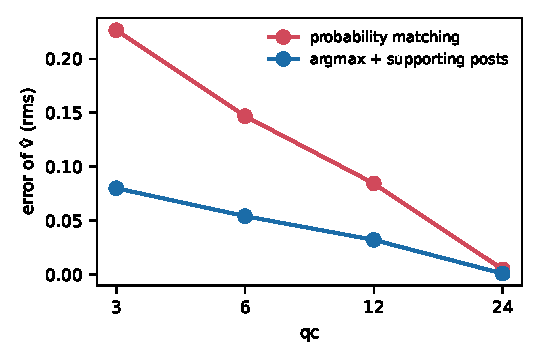
\includegraphics[width=0.45\linewidth]{figures/fig_sensing.pdf}
\caption{Error of $\hat v$ against the true share of all 24 agents, task003-nosolution.}
\label{fig:sensing}
\end{figure}

$\hat v$ is unbiased ($\pm 0.0005$), its error shrinks with $q_c$ and vanishes at
$q_c = 24$ (Figure~\ref{fig:sensing}). It is larger under probability matching because
those swarms stay mixed, which also makes gate mistakes more common: the controller
stays silent although the true share is below 0.75 on 5--8\% of nights, and posts
although it is above 0.75 on up to 13\% at $q_c = 3$. Abstaining agents (0.1--0.2\% of
agent-days) do not bias it.

\paragraph{Helping the truth versus agents' own proofs: does not apply here.} In
task003-symmetric, extra truth posts raise the share of agents holding a proof of A0 but
lower the share holding one from their own evidence. In task003-nosolution no proof is
possible by construction, so this question does not arise.

\paragraph{Caveats.} One world (task\_003), 24 agents, exact-Bayesian agents; means over
1,000 episodes per cell. Full analysis, code and tables:
\texttt{analysis/task003\_llm\_free/sim1\_analysis/} (reports Q0--Q6).

\end{document}
